\chapter{Teaching Online}\label{s:online}

\begin{quote}

  If you use robots to teach, you teach people to be robots. \\
  --- variously attributed

\end{quote}

Technology has changed teaching and learning many times. Before
blackboards were introduced into schools in the early 1800s, for
example, there was no way for teachers to share an improvised example,
diagram, or exercise with an entire class at once. Combining low cost,
low maintenance, reliability, ease of use, and flexibility, blackboards
enabled teachers to do things quickly and at scale that they had only
been able to do slowly and piecemeal before. Similarly, the hand-held
video camera revolutionized athletics training, just as the tape
recorder revolutionized music instruction a decade earlier.

Many of the people pushing the Internet into classrooms don't know
this history, and don't realize that it is just the latest in \href{http://teachingmachin.es/timeline.html}{a long
series of attempts} to use machines to teach
\cite{Watt2014}. From the printing press through radio and
television to desktop computers and mobile devices, every new way to
share knowledge has produced a wave of aggressive optimists who
believe that education is broken and that technology can fix
it. However, ed tech's strongest advocates have often known less about
``ed'' than they do about ``tech'', and have often been driven more by the
prospect of profit than by the desire to improve learning.

Today's debate is often muddied by the fact that ``online'' and
``automated'' don't have to be the same thing. Live online teaching
can be a lot like leading a small-group discussion. Conversely, the only
way to teach several hundred people at a time is to standardize and
automate assessment; the learner's experience is largely the same from
whether the automation uses software or a squad of teaching assistants
working to a tightly-defined rubric.

This chapter therefore looks at how the Internet can and should be used
to deliver automated instruction, i.e., to teach with recorded videos
and assess via automatically-graded exercises. The next chapter will
then explore ways of combining automated instruction with live teaching
delivered either online or in person.

\section{MOOCs}\label{s:online-moocs}

The highest-profile effort to reinvent education using the Internet is
the Massive Open Online Course, or MOOC. The term was invented by
David Cormier in 2008 to describe a course organized by George Siemens
and Stephen Downes. That course was based on a
\gref{g:connectivism}{connectivist} view of learning, which holds that
knowledge is distributed and learning is the process of finding,
creating, and pruning connections.

The term ``MOOC'' was quickly co-opted by creators of courses that kept
more closely to the hub-and-spoke model of a traditional classroom, with
the instructor at the center defining goals and the learners seen as
recipients or replicators of knowledge. Classes that use the original
connectivist model are now sometimes referred to as ``cMOOCs'', while
classes that centralize control are called ``xMOOCs''. (The latter kind of
course is also sometimes called a ``MESS'', for Massively Enhanced Sage on
the Stage.)

Two strengths of the MOOC model are that learners can work when it's
convenient for them, and that they have access to a wider range of
courses, both because the Internet brings them all next door and because
online courses typically have lower direct and indirect costs than
in-person courses. Five years ago, you couldn't cross the street on a
major university campus without hearing some talking about how MOOCs
would revolutionize education, destroy it, or possibly both.

But MOOCs haven't been nearly as effective as their more enthusiastic
proponents claimed they would be \cite{Ubel2017}. One reason is that
recorded content is ineffective for many novices because it cannot clear
up their individual misconceptions (Chapter~\ref{s:models}): if they
don't understand an explanation the first time around, there usually
isn't a different one on offer. Another is that the automated assessment
necessary in order to put the ``massive'' in MOOC only works well at the
lower levels of Bloom's Taxonomy. It's also now clear that learners have
to shoulder much more of the burden of staying focused in a MOOC, and
that the impersonality of working online can demotivate people and
encourage uncivil behavior.

\cite{Marg2015} examined 76 MOOCs on various subjects, and found that
the quality of lesson design was poor, though organization and
presentation of material was good. Closer to home, \cite{Kim2017}
studied 30 popular online coding tutorials, and found that they largely
teach the same content the same way: bottom-up, starting with low-level
programming concepts and building up to high-level goals. Most require
learners to write programs, and provide some form of immediate feedback,
but this feedback is typically very shallow. Few explain when and why
concepts are useful (i.e., they don't show how to transfer knowledge) or
provide guidance for common errors, and other than rudimentary age-based
differentiation, none personalize lessons based on prior coding
experience or learner goals.

\begin{aside}{Personalized Learning}

Few terms have been used and abused in as many ways as
\gref{g:personalized-learning}{personalized learning}. To most
ed tech proponents, it means dynamically adjusting the pace or focus
of lessons based on learner performance, which in practice means that
if someone answers several questions in a row correctly, the computer
will skip some of the subsequent questions.

Doing this can produce \href{https://www.rand.org/pubs/research\_briefs/RB9994.html}{modest
improvements} in outcomes, but
better is possible. For example, if many learners find a particular
topic difficult, the teacher can prepare multiple alternative
explanations of that point---essentially, multiple paths forward
through the lesson rather than accelerating a single path---so that
if one explanation doesn't resonate, others are available. However,
this requires a lot more design work on the teacher's part, which
may be why it's a less popular approach with the tech crowd.

And even if it does work, the effects are likely to be much less
than some of its advocates believe. A good teacher makes a
difference of 0.1--0.15 standard deviations in end-of-year
performance in grade school \cite{Chet2014} (see \href{http://educationnext.org/in-schools-teacher-quality-matters-most-coleman/}{this
article} for a brief summary). It's simply
unrealistic to believe that any kind of automation can outdo this
any time soon.

\end{aside}

So how should the web be used in teaching and learning tech skills? From
an educational point of view, its pros and cons are:

\begin{description}
\item[Learners can access more lessons, more quickly, than ever before.]
Provided, of course, that a search engine considers those lessons
worth indexing, that their internet service provider and government
don't block it, that the truth isn't drowned in a sea of
attention-sapping disinformation.
\item[Learners can access \emph{better} lessons than ever before,]
unless they are being steered toward second-rate material in order
to redistribute wealth from the have-nots to the haves
\cite{McMi2017}. (It's worth remembering that scarcity increases
perceived value, so as online education becomes cheaper, it will be
seen as being worth less.)
\item[Learners can access far more people than ever before as well.]
But only if those learners actually have access to the required
technology, can afford to use it, and aren't driven offline by
harassment or marginalized because they don't conform to the social
norms of whichever group is talking loudest. In practice, most MOOC
users come from secure, affluent backgrounds \cite{Hansen2015}.
\item[Teachers can get far more detailed insight into how learners work.]
So long as learners are doing things that are amenable to
large-scale automated analysis and either don't object to the use of
ubiquitous surveillance in the classroom, or aren't powerful enough
for their objections to matter.
\end{description}

\cite{Marg2015,Mill2016a,Nils2017} describe ways to accentuate the
positives in the list above while avoiding the negatives:

\begin{description}
\item[Make deadlines frequent and well-publicized,]
and enforce them, so that learners will get into a work rhythm.
\item[Keep synchronous all-class activities like live lectures to a minimum]
so that people don't miss things because of scheduling conflicts.
\item[Have learners contribute to collective knowledge,]
e.g., take notes together (Section~\ref{s:classroom-notetaking}),
serve as classroom scribes, or contribute problems to shared problem
sets (Section~\ref{s:individual-peer}).
\item[Encourage or require learners to do some of their work in small groups]
that \emph{do} have synchronous online activities such as a weekly online
discussion to help learners stay engaged and motivated without
creating too many scheduling headaches. (See
Appendix~\ref{s:meetings} for some tips on how to make these
discussions fair and productive.)
\item[Create, publicize, and enforce a code of conduct]
so that everyone can actually (as opposed to theoretically) take
part in online discussions (Section~\ref{s:classroom-coc}).
\item[Use lots of short lesson episodes rather than a handful of lecture-length chunks]
in order to minimize cognitive load and provide lots of
opportunities for formative assessment. This also helps with
maintenance: if all of your videos are short, you can simply
re-record any that need maintenance, which is often cheaper than
trying to patch longer ones.
\item[Use video to engage rather than instruct,]
since, disabilities aside, learners can read faster than you can
talk. The exception to this rule is that video is actually the best
way to teach people verbs (actions): short screencasts that show
people how to use an editor, step through code in a debugger, and so
on are more effective than screenshots with text.
\item[Identify and clear up misconceptions early]
(Chapter~\ref{s:models}). If data shows that learners are struggling
with some parts of a lesson, create alternative explanations of
those points and extra exercises for them to practice on.
\end{description}

All of this has to be implemented somehow, which means that you need
some kind of teaching platform. You can either use an all-in-one
learning management system like \href{http://moodle.org}{Moodle} or \href{https://www.sakaiproject.org/}{Sakai}, or
assemble something yourself using \href{http://slack.com}{Slack} or \href{https://zulipchat.com/}{Zulip} for
chat, \href{http://hangouts.google.com}{Google Hangouts} or \href{https://appear.in/}{appear.in} for
video conversations, and \href{https://wordpress.org/}{WordPress}, \href{http://docs.google.com}{Google
Docs}, or any number of wiki systems for collaborative
authoring. If you are just starting out, then use whatever requires
the least installation and administration on your side, and the least
extra learning effort on your learners' side. (I once ran a half-day
class using group text messages because that was the only tool
everyone was already familiar with.)

The most important thing when choosing technology is to \emph{ask your
learners what they are already using}. Normal people don't use
\href{https://en.wikipedia.org/wiki/Internet\_Relay\_Chat}{IRC}, and find its arcane conventions and interface
offputting. Similarly, while this book lives in a \href{http://github.com}{GitHub}
repository, requiring non-experts to submit pull requests has been an
unmitigated disaster, even with GitHub's online editing tools. As a
teacher, you're asking people to learn a lot; the least you can do in
return is learn how to use the tools they prefer.

\begin{aside}{Points for Improvement}

One way to demonstrate to learners that they are learning \emph{with} you,
not just \emph{from} you, is to allow them to edit your course notes. In
live courses, we recommend that you enable them to do this as you
lecture (Section~\ref{s:classroom-notetaking}); in online courses, you
can put your notes into a wiki, a Google Doc, or anything else that
allows you to review and comment on changes. Giving people credit for
fixing mistakes, clarifying explanations, adding new examples, and
writing new exercises doesn't reduce your workload, but increases
engagement and the lesson's lifetime
(Section~\ref{s:process-maintainability}).

\end{aside}

A major concern with any online community, learning or otherwise, is how
to actually make it a community. Hundreds of books and presentations
discuss this, but most are based on their authors' personal experiences.
\cite{Krau2016} is a welcome exception: while it predates the
accelerating descent of Twitter and Facebook into weaponized abuse and
misinformation, most of what was true then is true now.
\cite{Foge2005} is also full of useful tips for the community of
practice that learners may hope to join.

\begin{aside}{Freedom To and Freedom From}

Isaiah Berlin's 1958 essay ``\href{https://en.wikipedia.org/wiki/Two\_Concepts\_of\_Liberty}{Two Concepts of
Liberty}'' made a distinction between positive
liberty, which is the ability to actually do something, and negative
liberty, which is the absence of rules saying that you can't do
it. Unchecked, online discussions usually offer negative liberty
(nobody's stopping you from saying what you think) but not positive
liberty (many people can't actually be heard). One way to address
this is to introduce some kind of throttling, such as only allowing
each learner to contribute one message per discussion thread per
day. Doing this gives those with something to say a chance to say
it, while clearing space for others to say things as well.

\end{aside}

One other concern people have about teaching online is cheating.
Day-to-day dishonesty is no more common in online classes than in
face-to-face settings \cite{Beck2014}, but the temptation to have
someone else write the final exam, and the difficulty of checking
whether this happened, is one of the reasons educational institutions
have been reluctant to offer credit for pure online classes. Remote exam
proctoring is possible, usually by using a webcam to watch the learner
take the exam. Before investing in this, read \cite{Lang2013}, which
explores why and how learners cheat, and how courses can be structured
to avoid giving them a reason to do so.

\section{Video}\label{s:online-video}

A core element of cMOOCs is their reliance on recorded video lectures.
As mentioned in Chapter~\ref{s:performance}, a teaching technique called
Direct Instruction that is based on precise delivery of a well-designed
script has repeatedly been shown to be effective \cite{Stoc2018}, so
recorded videos can in principle be effective. However, scripts for
direct instruction have to be designed, tested, and refined very
carefully, which is an investment that many MOOC authors have been
unwilling or unable to make. Making a small change to a web page or a
slide deck only takes a few minutes; making even a small change to a
short video takes an hour or more, so the cost to the teacher of acting
on feedback can be unsupportable. And even when they're well made,
videos have to be combined with activities to be beneficial:
\cite{Koed2015} estimated, ``\ldots{}the learning benefit from
extra doing\ldots{}to be more than six times that of extra
watching or reading.''

If you are teaching programming, you may use screencasts instead of
slides, since they offer some of the same advantages as live coding
(Section~\ref{s:performance-live}). \cite{Chen2009} offers useful tips
for creating and critiquing screencasts and other videos;
Figure~\ref{f:online-screencasting} reproduces the patterns that paper
presents and the relationships between them, and is also a good example
of a concept map (Section~\ref{s:memory-concept-maps}).

\begin{figure}
\centering
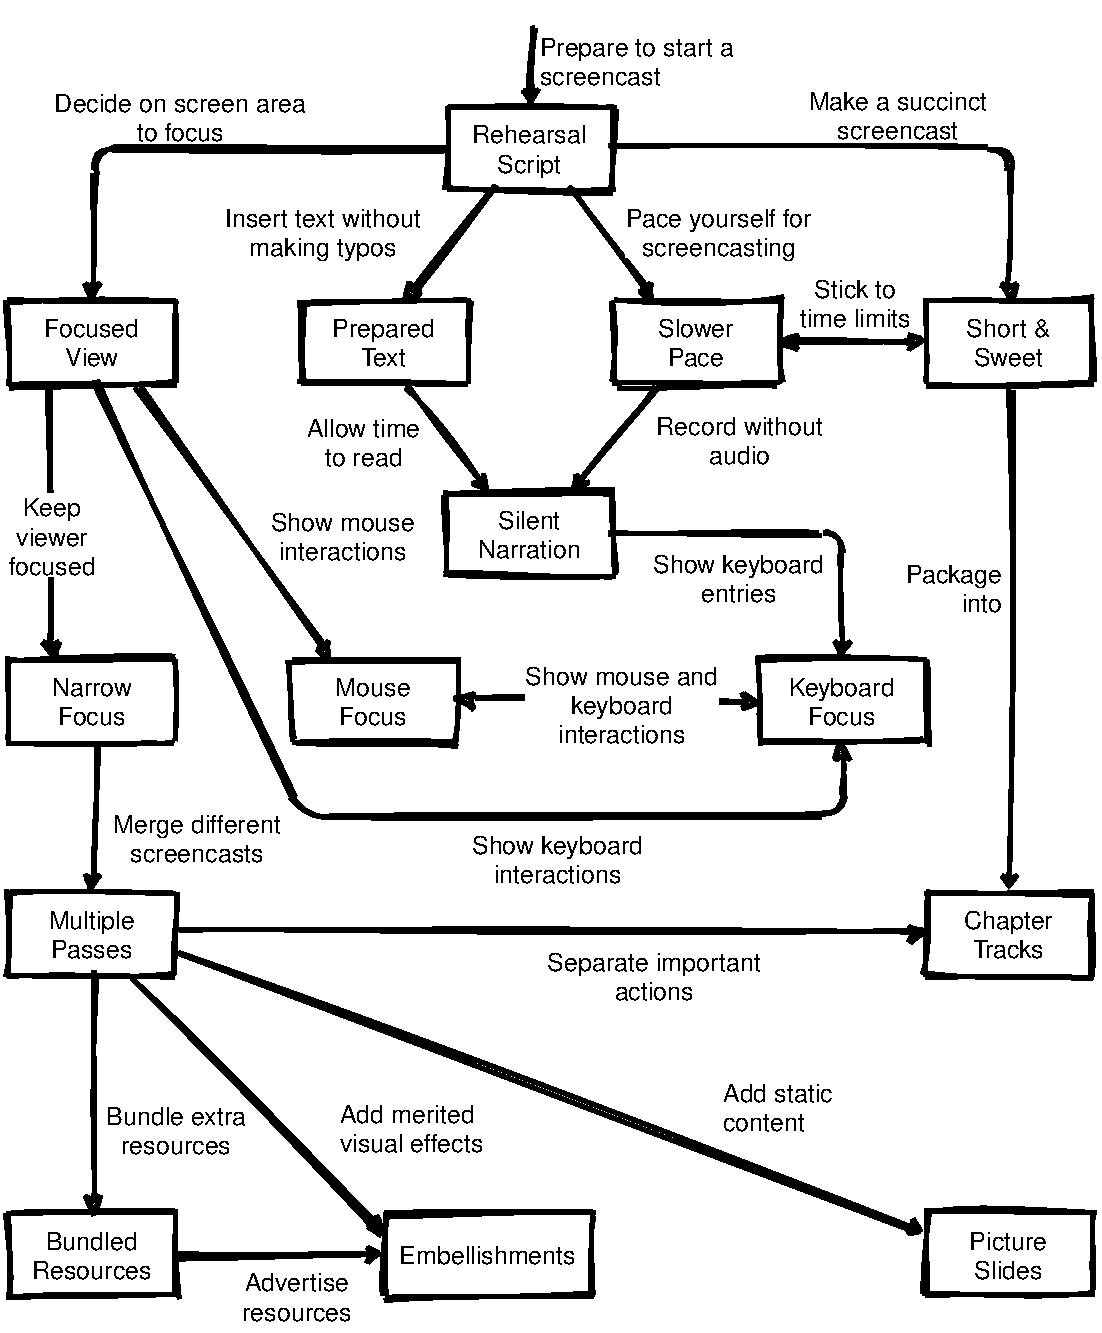
\includegraphics{../../figures/screencast.pdf}
\caption{Patterns for Screencasting ({[}Chen2009{]}(\#BIB))}
\label{f:online-screencasting}
\end{figure}

\cite{Guo2014} measured engagement by looking at how long learners
watched MOOC videos. Some of its key findings were:

\begin{itemize}
\item
  Shorter videos are much more engaging---videos should be no more than
  six minutes long.
\item
  A talking head superimposed on slides is more engaging than voice
  over slides alone.
\item
  Videos that felt personal could be more engaging than high-quality
  studio recordings, so filming in informal settings could work better
  than professional studio work for lower cost.
\item
  Drawing on a tablet is more engaging than PowerPoint slides or code
  screencasts, though it's not clear whether this is because of the
  motion and informality, or because it reduces the amount of text on
  the screen.
\item
  It's OK for teachers to speak fairly fast as long as they are
  enthusiastic.
\end{itemize}

One thing \cite{Guo2014} didn't address is the chicken-and-egg
problem: do learners find a certain kind of video engaging because
they're used to it, so producing more videos of that kind will
increase engagement simply because of a feedback loop? Or do these
recommendations reflect some deeper cognitive processes? Another thing
this paper didn't look at is learning outcomes: we know that learner
evaluations of courses don't correlate with learning
\cite{Star2014,Uttl2017}, and while it's plausible that
learners won't learn from things they don't watch, it remains to be
proven that they \emph{do} learn from things they \emph{do} watch.

\begin{aside}{I'm a Little Uncomfortable}

\cite{Guo2014}'s research was approved by a university research
ethics board, the learners whose viewing habits were monitored almost
certainly clicked ``agree'' on a terms of service agreement at some
point, and I'm glad to have these insights. On the other hand, I
attended the conference at which this paper was published, and the
word ``privacy'' didn't appear in the title or abstract of \emph{any} of the
dozens of papers or posters presented. Given a choice, I'd rather not
know how engaged learners are than see privacy become obsolete.

\end{aside}

There are many different ways to record video lessons; to find out which
are most effective, \cite{Mull2007a} assigned 364 first-year physics
learners to online multimedia treatments of Newton's First and Second
Laws in one of four styles:

\begin{description}
\item[Exposition:]
concise lecture-style presentation.
\item[Extended Exposition:]
as above with additional interesting information.
\item[Refutation:]
Exposition with common misconceptions explicitly stated and refuted.
\item[Dialog:]
Learner-tutor discussion of the same material as in the Refutation.
\end{description}

Refutation and Dialogue produced the greatest learning gains compared to
Exposition; learners with low prior knowledge benefited most, and those
with high prior knowledge were not disadvantaged.

\section{Flipped Classrooms}\label{s:online-flipped}

Fully automated teaching is one way to use the web in teaching; in
practice, almost all learning in affluent societies has an online
component: sometimes officially, and if not, through peer-to-peer back
channels and surreptitious searches for answers to homework questions.
Combining live and automated instruction allows instructors to use the
strengths of both. In a classroom, the instructor can answer questions
immediately, but it takes time for learners to get feedback on their
coding exercises (sometimes days or weeks). Online, it can take a long
time to get an answer, but learners can get immediate feedback on their
coding (at least for those kinds of exercises we can auto-grade).

Similarly, online exercises have to be more detailed because they're
anticipating questions. I find that in-person lessons start with the
intersection of what everyone needs to know and expands on demand, while
online lessons have to include the union of what everyone needs to know
because you aren't there to do the expanding.

The most popular hybrid teaching strategy today is the
\gref{g:flipped-classroom}{flipped classroom}, in which learners
watch recorded lessons on their own, and class time is used for
discussion and to work through problem sets. Originally proposed in
\cite{King1993}, the idea was popularized as part of peer instruction
(Section~\ref{s:classroom-peer}), and has been studied intensively over
the past decade. For example, \cite{Camp2016} compared students who
chose to take a CS1 class online with those who took it in person in a
flipped classroom. Completion of (unmarked) practice exercises
correlated with exam scores for both, but the completion rate of
rehearsal exercises by online students was significantly lower than
lecture attendance rates for in-person students. Looking at what did
affect the grade, they found that the students' perception of the
material's intrinsic value was only a factor for the flipped section
(and only once results were controlled for prior programming
experience). Conversely, test anxiety and self-efficacy were factors
only for the online section; the authors recommend trying to improve
self-efficacy by increasing instructor presence online.

But are lectures worth attending at all? Or should we just provide
recordings? \cite{Nord2017} examined the impact of recordings on both
lecture attendance and students' performance at different levels. In
most cases the study found no negative consequences of making recordings
available; in particular, students don't skip lectures when recordings
are available (at least, not any more than they usually do). The
benefits of providing recordings are greatest for students early in
their careers, but diminish as students become more mature.

\section{Life Online}\label{s:online-engagement}

\cite{Nuth2007} found that there are three overlapping worlds in
every classroom: the public (what the teacher is saying and doing), the
social (peer-to-peer interactions between learners), and the private
(inside each learner's head). Of these, the most important is usually
the social: learners pick up as much via cues from their peers as they
do from formal instruction.

The key to making any form of online teaching effective is therefore to
facilitate peer-to-peer interactions. To aid this, courses almost always
have some kind of discussion forum. \cite{Vell2017} analyzes
discussion forum posts from 395 CS2 students at two universities by
dividing them into four categories:

\begin{description}
\item[Active:]
request for help that does not display reasoning and doesn't display
what the student has already tried or already knows.
\item[Constructive:]
reflect students' reasoning or attempts to construct a solution to
the problem.
\item[Logistical:]
course policies, schedules, assignment submission, etc.
\item[Content clarification:]
request for additional information that doesn't reveal the student's
own thinking.
\end{description}

They found that constructive and logistical questions dominated, and
that constructive questions correlated with grades. They also found that
students rarely ask more than one active question in a course, and that
these \emph{don't} correlate with grades. While this is disappointing,
knowing it helps set instructors' expectations: while we might all want
our courses to have lively online communities, most won't.

Learners use forums in very different ways, and with very different
results. \cite{Mill2016a} observed that, ``\ldots{}procrastinators are
particularly unlikely to participate in online discussion forums, and
this reduced participation, in turn, is correlated with worse
grades. A possible explanation for this correlation is that
procrastinators are especially hesitant to join in once the discussion
is under way, perhaps because they worry about being perceived as
newcomers in an established conversation. This aversion to jump in
late causes them to miss out on the important learning and motivation
benefits of peer-to-peer interaction.''

\begin{aside}{Co-opetition}

\cite{Gull2004} describes an innovative online coding contest that
combines collaboration and competition. The contest starts when a
problem description is posted along with a correct, but inefficient,
solution. When it ends, the winner is the person who has made the
greatest overall contribution to improving the performance of the
overall solution. All submissions are in the open, so that
participants can see one another's work and borrow ideas from each
other; as the paper shows, the final solution is almost always a
hybrid borrowing ideas from many people.

\cite{Batt2018} described a small-scale variation of this used in
an introductory computing class. In stage one, each student submitted
a programming project individually. In stage two, students were paired
to create an improved solution to the same problem. The assessment
indicates that two-stage projects tend to improve students'
understanding, and that they enjoyed the process.

\end{aside}

Discussion isn't the only way to get students to work together online.
\cite{Pare2008} and \cite{Kulk2013} report experiments in which
learners grade each other's work, and the grades they assign are then
compared with grades given by graduate-level teaching assistants or
other experts. Both found that student-assigned grades agreed with
expert-assigned grades as often as the experts' grades agreed with each
other, and that a few simple steps (such as filtering out obviously
unconsidered responses or structuring rubrics) decreased disagreement
even further. And as discussed in Section~\ref{s:individual-peer},
collusion and bias are \emph{not} significant factors in peer grading.

\cite{Cumm2011} looked at the use of shareable feedback tags on
homework; students could attach tags to specific locations in coding
assignments (like code review) so that there's no navigational cost for
the reader, and they controlled whether to share their work and feedback
anonymously. Students found tag clouds of feedback on their own work
useful, but that the tags were really only meaningful in context. This
is unsurprising: the greater the separation between action and feedback,
the greater the cognitive load. What wasn't expected was that the best
and worst students were more likely to share than middling students.

\begin{aside}{Trust, but Educate}

The most common way to measure the validity of feedback is to compare
students' grades to experts' grades, but calibrated peer review
(Section~\ref{s:individual-peer}) can be equally effective. Before
asking learners to grade each others' work, they are asked to grade
samples and compare their results with the grades assigned by the
teacher. Once the two align, the learner is allowed to start giving
grades to peers. Given that critical reading is an effective way to
learn, this result may point to a future in which learners use
technology to make judgments, rather than being judged by technology.

\end{aside}

One technique we will definitely see more of in coming years is online
streaming of live coding sessions \cite{Haar2017}. This has most of
the benefits discussed in Section~\ref{s:performance-live}, and when
combined with collaborative note-taking
(Section~\ref{s:classroom-notetaking}) it can come pretty close to
approximating an in-class experience.

Looking even further ahead, \cite{Ijss2000} identified four levels of
online presence, from realism (we can't tell the difference) through
immersion (we forget the difference) and involvement (we're engaged but
aware of the difference) to suspension of disbelief (we are doing most
of the work). Crucially, they distinguish physical presence, which is
the sense of actually being somewhere, and social presence, which is the
sense of being with others. In most learning situations, the latter is
more important, and one way to foster it is to bring the technology
learners use every day into the classroom. For example,
\cite{Deb2018} found that doing in-class exercises with realtime
feedback using mobile devices improved concept retention and student
engagement while reducing failure rates.

\begin{aside}{Hybrid Presence}

Combining online and in-person instruction can be more effective than
either on its own. I have delivered very successful classes using
real-time remote instruction, in which the learners are co-located at
2--6 sites, with helpers present, while I taught via streaming video
(Section~\ref{s:joining-using}). This scales well, saves on travel
costs, and is less disruptive for learners (particularly those with
family responsibilities). What \emph{doesn't} work is having one group in
person and one or more groups remotely: with the best will in the
world, the local participants get far more attention.

\end{aside}

Online teaching is still in its infancy: \cite{Luxt2009} surveyed
peer assessment tools that could be useful in computing education, and
\cite{Broo2016} describes many other ways groups can discuss things,
but only a handful of these ideas are widely known or used.

\begin{quote}

  I think that our grandchildren will probably regard
  the distinction we make between what we call the real world
  and what they think of as simply the world
  as the quaintest and most incomprehensible thing about us. \\
  --- William Gibson

\end{quote}

\section{Exercises}\label{s:online-exercises}

\subsection*{Give Feedback on a Bad Screencast (whole class/20)}

Watch \href{https://youtu.be/xcnoHaxXvdQ}{this screencast} as a group and give
feedback on it. Organize feedback along two axes: positive
vs. negative and content vs. presentation. When you are done, have
each person in the class add one point to a 2x2 grid on a whiteboard
(or in the shared notes) without duplicating any points that are
already up there. What did other people see that you missed? What did
they think that you strongly agree or disagree with? (You can compare
your answers with the checklist in Section~\ref{s:checklists-teacheval}.)

\subsection*{Two-Way Video (pairs/10)}

Record a 2--3 minute video of yourself doing something, then swap
machines with a partner so that each of you can watch the other's video
at 4X speed. How easy is it to follow what's going on? What if anything
did you miss?

\subsection*{Viewpoints (individual/10)}

According to \cite{Irib2009}, different disciplines focus on
different factors affecting the success or otherwise of online
communities:

\begin{description}
\item[Business:]
customer loyalty, brand management, extrinsic motivation.
\item[Psychology:]
sense of community, intrinsic motivation.
\item[Sociology:]
group identity, physical community, social capital, collective
action.
\item[Computer Science:]
technological implementation.
\end{description}

Which of these perspectives most closely corresponds to your own? Which
are you least aligned with?

\subsection*{Helping or Harming (small groups/30)}

\href{https://www.nytimes.com/2018/01/19/business/online-courses-are-harming-the-students-who-need-the-most-help.html}{Susan Dynarski's article in the \emph{New York Times}}
explains how and why schools are putting students who fail in-person courses
into online courses, and how this sets them up for even further failure.

\begin{enumerate}
\item
  Working in small groups, read the article, come up with 2--3 things
  that schools could do to compensate for these negative effects, and
  create rough estimates of their per-student costs.
\item
  Compare your suggestions and costs with those of other groups. How
  many full-time teaching positions do you think would have to be cut
  in order to free up resources to implement the most popular ideas
  for 100 students?
\item
  As a class, do you think that would be a net benefit for the
  students or not?
\end{enumerate}

Budgeting exercises like this are a good way to tell who's serious about
educational change. Everyone can think of things they'd like to do; far
fewer are willing to talk about the tradeoffs needed to make change
happen.
